\documentclass[senior,final,11pt]{iscs-thesis}
%論文の種類とフォントサイズをオプションに
%\usepackage{graphicx}% 必要に応じて
%\usepackage{mysettings}% 自分用設定
%-------------------
\etitle{Neural Network based Decompiler for Machine Coding}
\jtitle{ニューラルネットを用いた機械語のための逆コンパイラ}

__NAMES__

\date{December 11, 2018}
%-------------------


\newcommand{\argmax}{\mathop{\rm arg\,max}\limits}
\newcommand{\argmin}{\mathop{\rm arg\,smin}\limits}

\usepackage{listings}
\usepackage{cite}
\usepackage{url}
\usepackage{natbib}
\usepackage[dvipdfmx]{graphicx}
\usepackage{framed}
\usepackage{caption}

\lstdefinestyle{myCustomMatlabStyle}{
  language=C,
  numbers=none,
  stepnumber=1,
  numbersep=10pt,
  tabsize=2,
  showspaces=false,
  showstringspaces=false
}

\lstdefinestyle{Csample}{
  language=C,
  tabsize=2,
 	framesep=5pt,
}

\lstdefinestyle{Asmsample}{
  tabsize=2,
  framesep=5pt,
  %frame=none,
}

\lstdefinestyle{ForDecomp}{
  tabsize=2,
  frame=l,
  framesep=5pt
}


\lstset{%
  basicstyle={\small},%
  commentstyle={\small\itshape},%
  keywordstyle={\small\bfseries},%
  % style={myCustomMatlabStyle},
  stringstyle={\small\ttfamily},
  breaklines=true,
  columns=[l]{fullflexible},%
  % frame={tb},
  % numbers=left,%
  xrightmargin=0zw,%
  xleftmargin=3zw,%
  numberstyle={\scriptsize},%
  stepnumber=1,
  numbersep=1zw,%
  lineskip=-0.5ex,%
  captionpos=b,
}



\begin{document}
\begin{eabstract}
A decompiler is a tool for recovering a source code from compiled binary data.
There are various decompilers, but they often output a source code that is not intelligible to humans. 
In this thesis, we apply machine translation techniques to generate human intelligible decompiled source codes. 
More specifically, we propose to use recurrent neural networks with attention, 
which have been demonstrated to be useful for machine translation. 
In experiments, we use source codes collected from open source projects and their binary data for training and evaluating the neural networks.
From the experiment, we can observe little improvement in the decompilation result with the use of attention.
However, the results were not applicable for practical use.

\end{eabstract}
\begin{jabstract}
逆コンパイラはコンパイル後のバイナリデータからソースコードを復元するためのツールである。
様々な逆コンパイラが存在するが、既存の逆コンパイラはしばしば人間にとって分かりにくいソースコードを出力する。
そこで本論文では、統計的機械翻訳の技術を逆コンパイラに用いた、解析者にとってわかりやすいソースコードを出力する逆コンパイラを提案する。
具体的には、機械翻訳において有用とされる注意機構付き再帰型ニューラルネットワークを用いる。
実験では、オープンソースプロジェクトから収集したソースコードとそのバイナリデータを用いてニューラルネットワークを学習し、その性能を検証した。
実験の結果、注意機構を用いることににより逆コンパイル結果における若干の精度向上が認められたが、実用的な精度までは至らなかった。
\end{jabstract}

\maketitle

\chapter{Introduction}
% For dinamic analysis, malware is executed in the sandbox and the behavior is examined with the changes ocuuring in the sandbox. 
% Usually, there are two malware analysis approach, the dinamic analysis and the static analysis.
% In the static analysys, the behavior of the malware is analyzed by 

These days, the amount of malware has been increasing rapidly. In the report of AV-TEST Institute,
over 100 million malwares are newly found in every year for the past five years \citep{malware_increase}.
There are many case studies for malwareinfection \citep{malware_case_1,malware_case_2,malware_case_3,malware_case_4}.
In those cases, they analyse malwares to assess the impact of the incident and to identify the vulnerability which causes the infection.
% Therefore, the importance of developing malware analysis tools has been rising.
% 要参考文献 -> つけた。
In order to analyse malwares quickly and efficiently, there are some tools for analysing malwares \citep{mal_anal_tool}.
One of these tools is a decompiler, which is a tool for analyzing the behavior of malware. 
This tool generates a C-like pseudocode which represents the behavior of the malware, and analysts can infer the behavior of the malware from the pseudocode.
This is much easier compared to analyzing raw binary codes.

However, sometimes a decompiler generates an unstructured code, which requires users to make an effort to understand the behavior of the program. 
This is due to flexibility of the high level language. If the decompiler chooses a human-friendly representation of the language as a result of decompiling, we can analyze malware with less effort. 

In this thesis, we apply neural networks to the problem of decompilation to generate human-friendly pseudocodes. 
This idea is originated from \cite{Motoneta}, in which they used recurrent neural networks, in particular sequence-to-sequence model, for decompilation.
However, their model does not seem to have some features for improving the quality of decompilation.
Therefore, we implemented the attention mechanisme, which is introduced in \cite{dot_attention}, for improving the quality.
Additionaly, the sequence-to-sequence model, which they used for modeling, ignores the structure of the C language code.
Therefore, we also implemented the sequence-to-tree model, which is suggested in \cite{Seq2Tree}, for generating structured C language source code.

In the experiment, we tested three models, the basic sequence-to-sequence model, the sequence-to-sequence model with attention and the sequence-to-tree model.
As the result of the experiment, the attention mechanism showed little improvemtn in the performance, while the sequence-to-tree does not.
Unfortunately, the results were not applicable for practical use, because the most of decompilation results were incorrect.

% In the following part of the paper, we explain the 

\chapter{Related Works}
In this section, we review related works.

\section{Decompilation with Machine Learning}

Because perfect decompilation is naturally impossible, there are some machine learning applications for decompilation.

In \cite{Motoneta}, they used the seqence-to-sequence model, which is a popular technique in the machine translation.
The seqence-to-sequence model is also evaluated in this thesis.

In \cite{genetic_decompiler}, they applied genetic programming to decompilation.
They prepared big corpus of C source codes, and they repeatedly mutated C code to reduce the difference of the target binary and the compilation result of the source code. 

% TODO(satos)

% Compiler and Optimization Level Estimation for Improving Anti-malware Technologies

% 

\section{Improvement of decompilation results}
In this thesis, we do not try to recover the function name and variable name. 
However, for hand-decompilation, sometimes the name can be estimated by the functionality of the variable.
For example, \cite{hand_decompilation} used Boomerang decompiler and repeatedly fixed variable types and names of the decompilation results 
to recover the source code of a software.

Here, we show a example of the name estimation.
Assume there is a variable X which seems to have a C struct type and has two fields P and Q.
Also, there are two functions F and G which operate with X. 
The function F receives X and another value V, assigns V to the memory indicated by P, adds 8 to P and increases Q. 
The function G receives X, subtracts 8 from P, decreases Q, and returns the value indicated by P.
In the situation, is is estimated that X has a name related to {\sl stuck}, the function F has a name related to {\sl push},
ands G has a name related to {\sl pop}.

\cite{name_recover_from_decompile_result} tackled this work. 
In that paper, they tried to estimate the name of a variable which appears in the decompilation result of a compiled C program.

This kind of name estimation also appears in the context of deobfuscation.
\cite{deobfsucation_matome}
% これ雑にreferenceしたけどあんま意味ないよなぁ...?
Deobfuscation is a reverse process of obfuscation.
Obfuscation is a technique to modify the program source code so that the code becomes hard to understand for humans. 
Obfuscation is used for hiding the behavior of a program whose source code has to be distributed.
For example, in the web application, a JavaScript code of a program should be distributed in order to be executed on client web browsers.
To protect the program from cracking, the JavaScript code is sometimes minified. All comments, newlines, indents are removed and variable names are substituted to automatically generated meaningless names. 

\cite{JSNaughty} applied statistical machine translation for this task. 
They calculated the future value of a variable from its functionality, then 
sought the most suitable name from the candidates generated from the corpus.

% 変数の性質から統計情報を取り出し、それを元に

\section{Neural Network for Program Generation}

There are many applications of neural networks for program synthesis. They are summurized in \cite{deep_programming_matome}.

In this thesis, we applied sequence-to-tree model suggested in \cite{Seq2Tree}, because the input of the decompiler is the sequence of machine codes.

For another example, in \cite{coffeescript_to_javascript}, they tried to mutually translate from JavaScript to CoffeeScript, and its inverse.
In that case, both JavaScript codes and CoffeeScript codes are tree structured, so they suggested tree-to-tree model.


\chapter{Problem Settings and Methots}

In this chapter, we explain about the statistical formalization of the decompilation problem,
and the neural network models used in the experiment.
\section{Decompiler}

% 320 words.

A compiler is a program which compiles a source code written in language X to another language Y. 
% 文献 Usually, X is a high-level language and Y is relatively a low-level language. 
For example, a Clang compiler translates the C language to the x64 assembly language, a javac compiler translates Java to a Java virtual machine code.
This process is usually 


A decompiler is a program which aims to reverse the process of a compiler, retrieving a source code of the high-level language X from a source code of a low-level language Y. 
% 文献
Especially, 
This reverse process is usually insufficient or impossible.
This is because a lot of informaition, such as variable names or function names, are lost when compiling.
Additionally, the program structure described in the high level-language is lost too. 
For example, a simple \texttt{for} statement can be represented by the combination of a \texttt{while} statement and an \texttt{if} statement, or the combination of \texttt{if} statement and \texttt{goto} statement. 
So a decompiler cannot distinguish the difference in their representations, 
although in the real situation \texttt{for} statement are often used and \texttt{goto} statement are rarely used.


% これについてちゃんと書く。
% Their output psudecodes are sometimes wrong or hard to understand.

% (DONE)表がはみ出しているのでどうにかした。

% \let\oldlstinputlisting\lstinputlisting
% \renewcommand{\lstinputlisting}[2][]{\oldlstinputlisting[frame=lines,#1]{#2}}

\begin{figure}
	\begin{tabular}{cc}
		\begin{minipage}[c]{0.5\hsize}
		\begin{framed}
			\lstinputlisting[breaklines=false]{insert_list.c}
			\end{framed}
			\caption*{Sample C source code}
		\end{minipage}
		\\
		\begin{minipage}[c]{0.5\hsize} %title={Result of the Hopper Decompiler}
			\begin{framed}
			\lstinputlisting[]{snowman.c}
			\end{framed}
			\caption*{Result of the Snowman Decompiler}
		\end{minipage}
		\begin{minipage}[c]{0.5\hsize}
			\begin{framed}
			\lstinputlisting[]{recstudio.c}
			\end{framed}
			\caption*{Result of the REC Studio Decompiler}
		\end{minipage}
	\end{tabular}
	\vspace*{-0.6cm}
	\caption{Decompilation results of existing decompilers for C source code}
	\label{fig:cw}
\end{figure}

Figure~\ref{fig:cw} shows an example of decompilation results of the Snowman decompiler version v0.1.3 and the REC Studio decompiler version 4.1 
for a sample C language code. The sample C code is compiled by the GNU C Compiler version 4.8.5, with the optimization level \texttt{-O0}.
The REC decompiler missed the structure of the variable \texttt{root}.
It also failed to estimate the number of arguments and the return value of the function.
The Snowman Decompiler succeeded to reconstruct the structure of the variable as \texttt{struct s0}.
It also succeeded to estimate the number of arguments and the return value as the semantically correct expressions, 
however the statement \texttt{return 0;} is reconstructed to the complex combination of statements.

These incorrect or verbose results might be due to missing patterns in the assembly codes. 
Existing decompilers are made up with many steps similarly to compilers \citep{decompiler_path,hex_rays}.
In each step, a decompiler finds patterns in binary data, converts them to more high-level structure.
However, covering all patterns might be hardly impossible, since there are many compilers and compiler optimizations.
文献欲しいが見当たらない...

Therefore, applying statical machine 


% These patterns comprehensive 

% The pathes are made up of 

% The \texttt{for} statement in the C source code is 
% reconstructed to the combination of the \texttt{while} statement and the {\sl if} statement in both decompiler results.

% This is the example of the impossibleness of the perfect decompilation, what we mentioned.



% However, there are many patterns 



% Existing decompilers are made up with many steps similarly to compilers. \citep{hex_rays,}
% They find patterns in binary data, convert them to more high-level structure, and chain them so that they can finally generate a high-level psudecode.



% このへん嘘書いてたので修正。
% The Hopper decompiler fails to detect while statements, and the variable {\sl now} is incorrectly analyzed.
% The output of snowman seems rather correct, as type {\sl struct tree} is reconstructed to {\sl struct s0}, 
% and the {\sl if} statement and {\sl while} statement are correctly restored. 
% However, it fails to detect the function epilogue, and the {\sl free} function call is incorrectly analyzed.
% Ideally, the decompilers can find correct function ranges and structure of statements, but they failed.


\section{Problem Settings}

% 189
In this thesis, we try to apply statistical approach, specifically SMT (statistical machine translation) technique, for decompilation.
The decompilation problem is formulated as follows. 

Given $sx = [sx_1, \dots, sx_n] $ as a tokenized sequence of the source code of domain language X, compiler generates $sy$ as a code of target language Y with probability $p(sy|sx)$.
Then, the best decompilation result for target source code $sy$ is $ \argmax_{sx} p(sx|sy)$. 
To generate $ \argmax_{sx} p(sx|sy)$, we decomposit $ p(sx|sy) = p([sx_1, \dots, sx_n] |sy) = \prod_{k=1}^{n} p(sx_k|sy,[sx_1,\dots,sx_{k-1}]) $,
where $ p(sx_k|sy,[sx_1,\dots,sx_{k-1}]) $ represents the probability that the token $ sx_k $ follows to the sequence $ [sx_1,\dots,sx_{k-1}] $ 
when the input sequence is $ sy $. 
We try to estimate the probability $ p(sx_k|sy,[sx_1,\dots,sx_{k-1}]) $ by LSTM, which is described in the next section.
With estimated $ p(sx_k|sy,[sx_1,\dots,sx_{k-1}]) $, we can generate approximated $ \argmax_{sx} p(sx|sy)$ sequentially from $sx_1$ to $sx_n$ by selecting token $ \argmax_{sx_{k}} p(sx_k|sy,[sx_1,\dots,sx_{k-1}]) $ at each timing.

% The LSTM is 
% We assume the prior distribution $p(sx)$ as the human-generated source code. 
% With that assumption, is in proportion to $p(sy|sx)p(sx)$ according to the Bayesian low, and 
% the $\argmax_{sx} p(sx|sy)$ is considered as the best human-intelligible decompilation result for the low-level code $sy$.  
% So we try to estimate $ \argmax_{sx} p(sy|sx)p(sx)$ for decompilation result.
% And if the compiler is deterministic, there would be a function $f$ which represents the compiler and $p(f(sx)|sx) = 1$,
% then the objective becomes to $ \argmax_{sx,f(sx)=sy} p(sx)$.

% The distribution $p(sx)$ is approximated by collecting source code from open source projects.
% So if we had enough high-level source code data, we could choose the most popular high-level source code which generates given low-level code for the decompile result.
% However, high-level source code data can't be comprehensive.
% So we have to model the structure of compilation process somehow.
% We modeled the structure by the LSTM, which is commonly used in resent SMT techniques.

\section{Modeling}

% (TODO)LSTM,Seq2seqの説明、その後Attentionについて説明、さらにその後seq2treeについて説明する。
\subsection{LSTM}
%72 words.
LSTM (Long Short-Term Memory) is a unit of Recurrent Neural Network. 
It is first introduced in \cite{first_LSTM}, for overcoming the vanishing gradient problem and exploding gradient problem.
Roughly speaking, LSTM unit recieves two input vectors, 
the one represents the internal state of the LSTM, and the other is the input for the LSTM unit, 
and LSTM emits one output vectors, which represents the next internal state of the LSTM.

\subsection{Sequence-to-Sequence}
% This model is called seq2seq (sequence to seqence) model.

% 477 words.
LSTM unit is applied for SMT task in \cite{seq2seq}, as the essential unit of the sequence-to-sequence (sequence to sequence) model.
SMT is the task which tries to translate one sentense $sx$ written in one language into the sentense $sy$ written in another language.

Sequence-to-sequence model is composed of two modules, the encoder netwrok and the decoder network.

The purpose of the encoder network is to summerize the input sequence $sx$, whose length varies depending on the sequence, into one fixed length vector.
This process is carried out as follows. 
First, $sx$ is tokenized to sequence $sx_{1} \dots sx_{n}$, and each token $sx_{k}$ is embedded to its vector representation $vx_{k}$. 
Then, the initial LSTM internal state $enc_0$ is intialized randomely, 
and $ enc_{1} \dots enc_{n} $ are calculated in accordance with the recursive formula $ enc_{k} = lstm_{enc}(enc_{k-1},vx_{k}) $.
Finally, the last internal state $ enc_{n}$ is returned as the reduced representation of the input sequence $sx$.

The purpose of the decoder network is to estimate the distribution $ p(sy_k|sx,[sy_1,\dots,sy_{k-1}]) $. 
The training process is carried out as follows. 
First, $sy$ is tokenized, appended the token $ EOS $ for indicating the end of the sequence, then embedded to a vector representation $vy_{1} \dots vy_{m}$ in the same way as embedding $sx$.
From the start vector $y_{begin}$ and encoded input $ enc_{n} $, first internal state $ dec_{1}$ is calcuated as $ LSTM_{dec}(enc_{n},y_{begin}) $.
Then, $ dec_{1} \dots dec_{m} $ are calculated in accordance with the recursive formula $ dec_{k} = lstm_{dec}(dec_{k-1},vy_{k}) $.
Each decoder internal state $ dec_{k} $ is passed to the linear layer $ W_{dec} $ and then softmaxed to generate a probability vector $ py_{k} $.
The probability vector $ py_{k} $ is intended to represent the probability distribution $ p(sy_k|sx,[sy_1,\dots,sy_{k-1}]) $.
So the network is trained to reduce the difference between predicted distribution $ py_{k} $ and actual distribution $ p(sy_k|sx,[sy_1,\dots,sy_{k-1}]) $.
In the experiment, we choiced cross-entropy of $ py_{k} $ and $ p(sy_k|sx,[sy_1,\dots,sy_{k-1}]) $ for loss function.

The inference for sequence $sx$ is carried out by calculating 
$ \argmax_{sy} p(sy|sx) = \argmax_{sy} \prod_{k=1}^n p(sy_k|sx,[sy_1,\dots,sy_{k-1}]) $.
Calculating argmax directly is time consuming, so we have to approximate the argmax by calculating $sy = [sy_1, \dots sy_m]$ sequentially.
First, $sy_1$ is calculated as $ \argmax_{sy_1} p(sy_1|sx,[]) $, where distribution $ p(sy_1|sx,[]) $ is approximated by 
$ softmax(W_{dec}(dec_{1}))$. 
Then, the next token $sy_2 = \argmax_{sy_1} p(sy_2|sx,[sy_2]) $ is calculated from $ dec_{1} $ and the vector embedding of $sy_1$, and so on.
When the token $sy_{m+1}$ is the $ EOS $ token, generating process is stopped and the sequence $ [sy_1, \dots sy_m]$ is returned as the inference result.

% ビームサーチ書く。
% For TODO

% (TODO) このへんで 図を入れる
% (TODO) 理由/気持ち について述べたいですね。

What is mentioned above is the basic structure of the sequence-to-sequence model.
To improve the performance of the sequence-to-sequence model, there are some devices for the model.
In the following, we introduce two devices, which are used in our experiment.

First is the Bidirectional Reccurent Neural Networks (BRNN) is the architecture introduced in \cite{BiRNN}.
In the experiment, this architecture is used for the encoder network as follows.
In addition to the internal state $ enc_{k} $, the reverse internal state $ enc_{k}^{\gets} $ is also calculated 
in accordance with the recursive formula $ enc_{k}^{\gets} = lstm_{enc}^{\gets}(enc_{k+1}^{\gets},vx_{k}) $.
Then both of the internal states $ enc_{n} $ and $ enc_{1}^{\gets} $ are used for decoder network.

Second is the multi-layer reccurent neural networks, introduced in \cite{multi_layer}.
They reported that, feeding the output sequence of the LSTM network to another LSTM network, like stucking the network layers, will improve the accuracy of the prediction.
This architecture is called as stucked reccurent neural networks or multi-layer reccurent neural networks.



% It is reported that, instead of the output of the LSTM units to another LSTM units will improve the accuracy of the prediction.
% This architecture is called as stucked reccurent neural networks or multi-layer reccurent neural networks.


\subsection{Attention}
Attention is a extension module for sequence-to-sequence model to improve the quality of translation. 
Simple sequence-to-sequence model has a problem that the length of the encoded vector $enc_{n}$ is fixed 
regardless of the length of the input sequence $sx$. 
Therefore, the longer the length of the input becomes, the more likely the information of the input will be lost.
This problem is eased by using the information in the encoding network when decoding the output sequence.

The attention module is first developed by \cite{attention_paper}.
We inplemented the global general attention, which is intoduced in \cite{dot_attention}, for improving the quality of decompilation.
In the following, we will describe about the global general attention.

As above mentioned, the pure sequence-to-sequence model uses the output of decoder network $ dec_{k} $ for estimating 
the distribution $ p(sy_k|sx,[sy_1,\dots,sy_{k-1}]) $.
In the sequence-to-sequence model with attention, 
a context vector $ ctx_{k} $ is calculalted from $ dec_{k} $ and the internal states of encoder network $ enc_{1} \dots enc_{n} $, 
then the distribution is estimated from the output vector $ dec_{k} $ and context vector $ ctx_{k} $.
The context vector $ ctx_{k} $ is calculated as follows.
For each state $ enc_{l} $, the importance of the state $ a_{l} $ is calculalted as $ a_{l} = score(dec_{k},enc_{l}) $,
then the $ ctx_{k} $ is calculated as $ ctx_{k} = \sum_{l=1}^{n} \frac{\exp{a_{l}}}{\sum_{l=1}^{n}\exp{a_{l}}} enc{l} $, as the weighted average of $ enc_{1} \dots enc_{n} $.
% Multiple score functions are introduced by \cite{dot_attention}, and we choiced 
In the paper by \cite{dot_attention}, various kinds of score function is suggested.
We used general score function, which is calculated as $ score(dec_{k},enc_{l}) = dec_{k}^T W enc_{l} $ ,
where W is the parameter matrix. 

% With the information of the internal state $ ctx_{k} $ of the encoder network, the decoder network can access to the 

% アテンション機構を用いる場合、前述したようにdecoder networkの出力 $ dec_{k} $ をそのまま用いて分布をesitmateするのではなく、
% $ dec_{k} $ と encoder network の出力 $ enc_{1} \dots enc_{n} $ (encoder が BiLSTMの場合 $ enc^{\gets}_{1} \dots enc^{\gets}_{n} $ も)
% を用いて context vector $ ctx_{k} $ を生成し、 $ dec_{k} $ と $ ctx_{k} $ によって条件付き分布をesitmateする。

% $ ctx_{k} $ は、 $ enc_{1} \dots enc_{n} $ の加重平均によって計算される。 具体的には、
% 各状態 $ enc_{l} $ について その状態のスコア $ a_{l} = score(dec_{k},enc_{l}) $ を計算し、
% $ ctx_{k} = \sum_{l=1}^{n} \frac{\exp{a_{l}}}{\sum_{l=1}^{n}\exp{a_{l}}} enc{l} $ として計算される。

% この $ ctx_{k} $ を併せて用いることにより、 分布予測時に入力データの情報にアクセスすることができ、精度の向上が見込める。


% In the pure sequence-to-sequence model, the conditional probability  $ p(sy_k|sx,[sy_1,\dots,sy_{k-1}]) $ is calculated from $ dec_{k} $ ,which is the internal state of the decoder network.
% In the sequence-to-sequence with attention model, the probability is calcutated from $ dec_{k} $ and the context vevctor $ c_{k} $.
% $ c_{k} $


% After generating $ dec_{k} $, the context vector $ c_{k} $ is calculated from the hidden states $ enc_{1} \dots enc_{n} $.

% $ c_{k} = \sum_{k=1}^{n} $ 

% The attentional hidden state $ dec'_{k} $ is calculated from the $ dec_{k} $ and $ c_{k} $.
% Then, the probability $ p(sy_k|sx,[sy_1,\dots,sy_{k-1}]) $ is estimated as $ softmax(W_{dec}(dec'_{k}))$, instead of $ softmax(W_{dec}(dec_{k}))$.




\subsection{Sequence-to-Tree}
% 184 words
Compare to natural languages, programming languages obeys rigid grammers. % wich are usually context free grammers.
Therefore, it is reasonable to consider the grammer of the programming language when generating programs.
Sequence-to-Tree is a model for generating tree-structured output from sequence input. 
This model is introduced in \cite{Seq2Tree} for generating a program from a program specification written in the natural language. 
This task is similer to our task, which aims to generate programs from the sequence of the assembly code, so we implemented this model in the experiment.

Now, we will describe about the sequence-2-tree model.
sequence-to-tree model is composed of two modules, the encoder netwrok and the decoder network.
The encoder network of sequence-2-tree model is the same as the encoder network of sequence-to-tree model. It summerize the input sequence into one fixed length vector.

\begin{figure}[]
	\begin{center}
	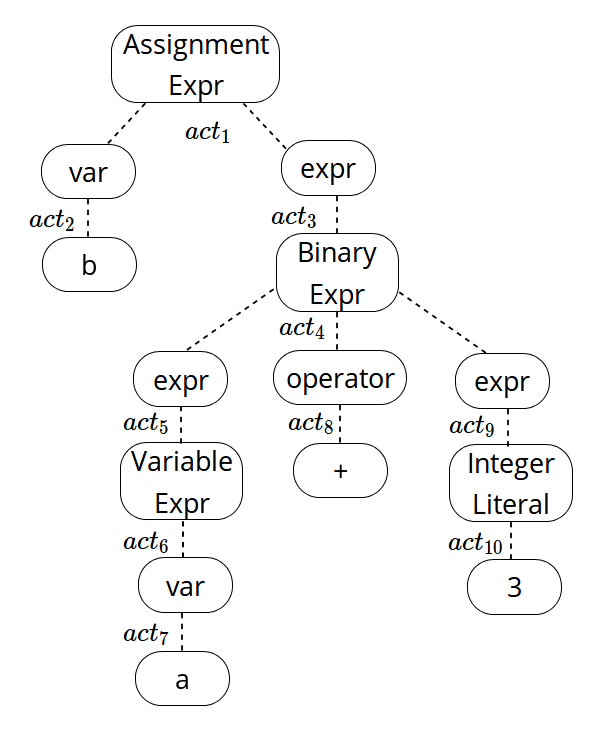
\includegraphics[height=12cm]{ast_zu.png}
	\end{center}
	\caption{AST representation of a C statement \texttt{b = a + 3;} }
	\label{fig:ast_zu}
\end{figure}

The decoder network is a network for generating tree structured output. 
A tree-structure is representable by the sequence of the actions which expands a nonterminal symbol of the constructing tree.
For example, the tree shown in figre~\ref{fig:ast_zu} is gererated from the sequence $ [act_1, \dots act_{12}] $, 
where action $ act_k $ expands the left-most nonterminal symbol in the tree generated from the action sequence $ [act_1, \dots act_{k-1}] $. 
Suppose the tree $ty$ is generated by the action sequence $ [act_1, \dots act_m] $, 
then the tree-generating probability $ p(ty|sx) $ is decomposed to $ \prod_{k=1}^n p(act_k|sx,[act_1, \dots act_{k-1}]) $. 
The sequence-to-sequence model is now applicable for generating tree structure, by emmbeding each action to representing vector $av_k$ and 
calculating $ LSTM_{dec}(dec_{k},av_{k}) $ sequentially for estimating $p(act_{k+1}|sx,[act_1, \dots act_{k}]) $.  

% In algorithmic parspective, the inference of the seq2seq model tries to generate sequence one by one, from the first token to the last.
% The Seq2Tree model also tries to generate tree structure one by one, with depth-first order.
% The inference of the SeqTree model starts from the start symbol, and recursively expand the nonterminal symbols in depth-first order.

In that paper, they additionaly tries to use the information which is peculiar to the tree structure. 
For expanding the node $d$, they also use the information of node type $ nf_{d} $ and the parent action $p_{d}$ from which $d$ is generated.
And they calculalte $ LSTM_{dec}(dec_{k},[av_{k}; nfv_{d}; pv_{d}]) $ instead of $ LSTM_{dec}(dec_{k},av_{k}) $, 
where $nfv_{d},pv_{d}$ are the vector embedding of $nf_{d},p_{d}$.

They also used devised method for generating terminal symbols, because they need to copy the name of some variables from the program specification.
However, in our case, we do not need copy the information from the input, because the name information is lost when compiling.
Nevertheless, it is found from the experiments that our decompilers often fail to recover the constant values in the programs.
Therefore, implementing the copying method is left for future work.

% しかしながら、実験の結果、ソースコード中の定数に関しては復元が困難であることが観察された。このため、プログラム中の定数に関してこのcopy method を実装することが考えられるが、
% これは future work とする。

% \subsection{Path Decomposite Sequence-to-Tree}
% 前述の Sequence-to-Tree は プログラムの構造を考慮しているものの、アクションをそのまま列にするのは結局プログラムの木としての構造がある程度失われてしまっているのではないかと考えられる。
% すなわち、アクションを列に展開しているため、ある部分木からその兄弟の部分木の生成に移る際に大幅なジャンプが生じている。

\chapter{Experiments}
In this chapter, we explain the detail of the data preparetion and implementation.
The implementation source codes are avaiable at \url{https://github.com/satos---jp/neural_decompiler}.  

\section{Data Collection}
% 219 words
First, we collected source codes by crawling \cite[GitHub]{github}, cloning about 900 repositories with C language topic, 
and recursively searched each folder to enumerate C language source code.
From each source code, we generated pairs of C source code fragment and x64 assembly code corresponds to the C fragment.
Some example data pairs are shown in figure~\ref{fig:pairsoffragments}. 

\begin{figure}
	\begin{tabular}{|l|l|} \hline
	 C source code & x64 assembly \\ \hline 
		\begin{lstlisting}[style=Csample]
		r *= a
		\end{lstlisting}
		&
		\begin{lstlisting}[style=Asmsample]
	mov eax,DWORD [rbp-0x4]
	imul eax,DWORD [rbp-0x14]
	mov DWORD [rbp-0x4],eax
		\end{lstlisting} \\ \hline	
		\begin{lstlisting}[style=Csample]
	while(p >= 0){
		p--;
		r *= a;
	}
		\end{lstlisting}
		&
		\begin{lstlisting}[style=Asmsample]
	jmp LABEL_0
LABEL_1 :
	sub DWORD [rbp-0x18],0x1
	mov eax,DWORD [rbp-0x4]
	imul eax,DWORD [rbp-0x14]
	mov DWORD [rbp-0x4],eax
LABEL_0 :
	cmp DWORD [rbp-0x18],0x0
	jns LABEL_1
		\end{lstlisting} \\ \hline		
		\begin{lstlisting}[style=Csample]
int pow(int a,int p){
	int r = 1;
	while(p >= 0){
		p--;
		r *= a;
	}
	return r;
}
		\end{lstlisting}
		&
		\begin{lstlisting}[style=Asmsample]
	push rbp
	mov rbp,rsp
	mov DWORD [rbp-0x14],edi
	mov DWORD [rbp-0x18],esi
	mov DWORD [rbp-0x4],0x1
	jmp LABEL_0
LABEL_1 :
	sub DWORD [rbp-0x18],0x1
	mov eax,DWORD [rbp-0x4]
	imul eax,DWORD [rbp-0x14]
	mov DWORD [rbp-0x4],eax
LABEL_0 :
	cmp DWORD [rbp-0x18],0x0
	jns LABEL_1
	mov eax,DWORD [rbp-0x4]
	pop rbp
	ret
		\end{lstlisting} \\ \hline
	\end{tabular}
	\caption{Example of training data pairs}
	\label{fig:pairsoffragments}
\end{figure}

The pairs were generated as follows. Let {\sl S0} be an original C source code.
\begin{enumerate}
\item Remove all preprocessor, such as {\sl \#include}, in {\sl S0} to generate preprosessed C code {\sl S1}. 
\item Tokenize {\sl S1} and rearrange them in {\sl S2} so that there is exactly one token for each line. 
\item 
Compile {\sl S2} by gcc (GNU C compiler) with no optimization (-O0) and debug option to get assembly code {\sl S3}. 
With debug option, {\sl S3} contains information about the source code position which each assembly operations are originated from.
\item Assemble {\sl S3} to object file {\sl S4} and disassemble {\sl S4} to get information eliminated assembly code {\sl S5}.
\item 
Parse {\sl S2} with clang to get AST (abstract syntax tree) of the source code. 
And for each subtree of AST, we can get C fragment source code which corresponds to the subtree, 
and we can get assembly code corresponds to the C fragment by employing {\sl S5} combine with {\sl S3}.
\end{enumerate}

The C fragment and assembly code pairs are preprocessed for the training and testing data.


\section{Data Preprocessing}

% 34 words
In order to apply LSTM, input and output for the LSTM must be the sequence of tokens. 
So we have to preprocess the assembly data and C fragments to the token sequences by somehow.

\subsection{Assembly Code Preprocess}
% 155 words
There are two ways for preprocessing assembly codes.

First way is the raw binary integers. The assemblies are finally assembled to the sequence of the one byte integers, ranged from 0 to 255.
So the one byte integer sequences can be directly used for input sequences.

Second way is the tokenized sequence of assembly codes. 
The disassembled opcodes and operands in {\sl S5} are split to symbols, and concatenated these sequences to one sequence, then we modified followings.
\begin{itemize}
\item For each end of the operations, the {\sl ENDLINE} symbol is added to indicate the end of operation.
\item 
The relative access of code address, such as {\sl call} or {\sl jump} operations, 
are relabeled like $\alpha$-conversion for making code position independent and for reducing the vocabulary size.
\item The big integer values are substituted. 
In detail, the integer in the range from -255 to 256 are preserved as it is, and the other integeres are substituted with the {\sl \_\_HEX\_\_} symbol.
This also reduces the vocabulary size.
\end{itemize}

We choiced second way for the experiment.
This is because, in our case, the assembly code is generated from common C compiler, therefore the assembly code can be disassembled uniquely.
For example, \cite{disasm_obfuscate} proposed a obfuscation technique, which deceives the disassembler to generate wrong disassembly result.
In that case, the first way might be better than the second way.

\subsection{C Code Preprocess}
% 232 words
The C source codes were parsed to AST by the \cite{clang} and its Python bindings together with \cite{pycparser}, 
because all of the tools are individualy not sufficient for generating dataset.
Then, the AST is converted to input data by following modifications.

\begin{itemize}
\item The variable-ary nodes and optional nodes are converted. 
For example, the {\sl CompoundStatement} node has variable number of statements. 
We converted such list of nodes to the chains of concatnation {\sl CONS} and termination {\sl NIL}, like a list representation in functional language.
Another example is the  {\sl If} statement, whose {\sl else} clausure are sometimes missing. 
We converted such optional node to the alternative of {\sl SOME} and {\sl NONE}, like a optional data structure in functional language.
\item The variable names, function names, label names, or type names were renamed like $\alpha$-conversion.
\item There are four type of literals in C language. 
The integer literal less than 256 is preserved, and the literal greater than 256 is clipped to 256.
The string, float and character literals are converted to {\sl \_\_LITERAL\_\_} simbol.

Modifying the node to indicate the value in the assembly code corresponding to the literal is also conceibable way,
but we did not implement this because of its technical difficalty, so this is left to future work.
\end{itemize}

The AST is used for sequence-to-Tree model dataset as it is.
Also, the AST is converted to C token sequence for sequence-to-sequence model dataset. 

\section{Model Configuration}
The training model was implemented with Chainer version 4.5.0. (\url{https://chainer.org/})
We implemented three models, Seq2seq, Seq2seqAtt, and Seq2tree.

The encoder module was bidirectional LSTM in all of three models.
The decoder module of Seq2seq and Seq2seqAtt predict the conditional probability of a next token $ p(sy_k|sx,[sy_1,\dots,sy_{k-1}]) $,
while the decoder module of Seq2tree predicts the conditional probability of a next action $ p(a_{k}|sx,[a_1, \dots a_{k-1}]) $.

Seq2seqAtt and Seq2tree are the models with attention, while Seq2seq is not.

\begin{figure}[h]
	\begin{tabular}{|c||c|c|c|}
		\hline
		  & Seq2seq & Seq2seqAtt & Seq2tree \\ \hline \hline
		 Generate & \multicolumn{2}{|c|}{token sequence} & AST \\ \hline
		 With Attention & no & \multicolumn{2}{|c|}{yes} \\ \hline
		 Encoder & \multicolumn{3}{|c|}{Bidirectional LSTM} \\ \hline
		Number of LSTM Layers & \multicolumn{3}{|c|}{4} \\ \hline
		Dimensionality of Vector Embedding & \multicolumn{3}{|c|}{128} \\ \hline
	\end{tabular}
	\caption{The configuration parameters of the models}
	\label{fig:parameterofmodels}
\end{figure}

Figure~\ref{fig:parameterofmodels} shows the parameters of the models. 

% (TODO)レイヤ数、ロスについてのべる。

\section{Model Training}
% 91 words
We trained the model to reduce the cross-entropy loss between predicted and actual conditional probability.
The conditional probability is the probability of next token $ p(sy_k|sx,[sy_1,\dots,sy_{k-1}]) $ for sequence-to-sequence model, 
and the probability of next action $p(a_{k+1}|sx,[a_1, \dots a_{k}]) $ for sequence-to-tree model.

For the optimizer of the training, we used Adam, which is introduced in \cite{Adam}.
The paremeters of Adam are $ (\alpha,\beta_1,\beta_2) = (0.001,0.9,0.999) $, which are the default parameters of Chainer version 4.5.0.
% 学習の際のoptimizerにはAdam(文献)を用いた。

\section{Model Evaluation}
We evaluated the quality of the decompilation by two metrics, edit distance ratio and BLEU.

Edit distance ratio is the metrics for the correctness of the decompilation result.
Here, the edit distance ratio between two strings means the Levenshtein distance divided by the average length of the two strings.
Idealy, the correctness of the decompilation result should be measured by the distance of the meaning of the program.
However the decompilation result is usually uncompilable, so we used the edit distance of the source codes as the approximation of the correctness.

BLEU is the metrics for the similality of the ground truth and the decompilation result. 
It is first introduced in \cite{BLEU}, for evaluating the performance of the machine translation.
BLEU is calculated from the sets of the n-gram for each sentense. 
If the two sentens has similar n-gram sets, the BLEU score becomes higher.
In our case, it means that the decompilation result is more similer to the program written by human, that is, more human intelligible.

% 2つの文のn-gram集合が似ているほど、BLEUスコアは高くなります。今回の場合はデコンパイル結果がより人間らしい自然な出力となっていることを意味します。

In the experiment, we normalized variable names in the source codes by renaming. 
% 補足として、今回は edit distance と BLEU を計算する際に、変数名を先頭から順に順番に付け直すことにより、ソースコード中の変数名の付けなおしを行っている。
% これはプログラムの意味は変数名に依らないためである。

\chapter{Evaluation}
In this chapter, we show the evaluated result of the three models, Seq2seq, Seq2seqAtt, and Seq2tree.
% We trained each models with reedbush, を用い、各モデルについて4時間学習させた。
% We collected approximately $ 10^7 $ pairs of datasets. 

% \section{Furure work}

% TODO(satos)

% At first, we show the 

% まず先に、学習に用いたデータ長の分布を Figure~\ref{fig:editdist} に示す。
% ソースコードの部分木を全て列挙するデータ生成法の性質上、長さの短いコード辺が極端に多いことが確認できる。

% We tested three models. 

% 今回、それぞれのモデルの学習には、東京大学のreedbushを用い、各モデルについて4時間学習させた。

% 精度計測では、各モデルに対して テストケースから100個のデータをランダムに取り出して翻訳させ、それらの編集距離とBLEU値の平均を計測した。

\section{Numerical Evaluation}
For evaluating each model, we randomly sampled 100 data pairs from test cases, generated estimated decompilation results for each test cases,
then averaged the edit distance ratios and BLEU scores between results and ground truths.

\begin{figure}[]
	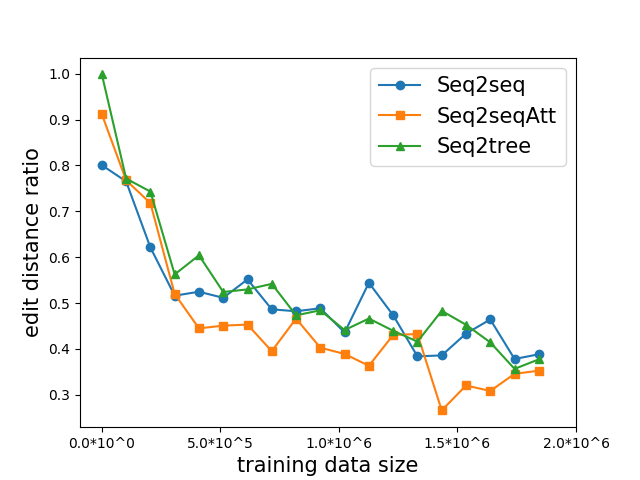
\includegraphics[width=12cm]{edit_dist.png}
	\caption{Averaged edit distance ratio for each models}
	\label{fig:editdist}
	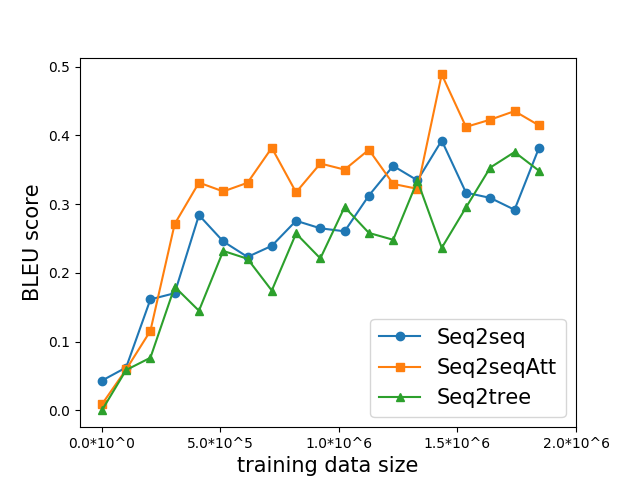
\includegraphics[width=12cm]{bleu.png}
	\caption{Averaged BLEU score for each models}
	\label{fig:bleu}
\end{figure}

% 図1は各モデルについて、学習に用いたデータ数と編集距離をプロットしたグラフである。
% 図2は各モデルについて、学習に用いたデータ数と編集距離をプロットしたグラフである。
Figure~\ref{fig:editdist} shows the relation of trainig data size and the averaged edit distance ratio for each models.
Figure~\ref{fig:bleu} shows the relation of trainig data size and the averaged BLEU score for each models.
The lower edit distance ratio and the higher BLEU score means the better decompilation performance.

We can see that Seq2seqAtt shows slightly better results in both edit distance ratios and BLEU scores,
 which implies that the attention improves the performance of the decompilation.
However, there are no significant difference between Seq2seq and Seq2tree in both metrics.
This seems to be due to the length of the sequences to be estimated.
% Seq2seqの結果とSeq2seqAttの結果を比較することにより、attention が性能向上に寄与していることがわかります。
% 逆にSeq2treeにはattentionがあるにもかかわらずSeq2seqと比較して性能向上が見られなかったわけですが、
% これはCのソースコードをASTに変換した際に、データサイズが増えたためであると考えられます。

\begin{figure}[]
	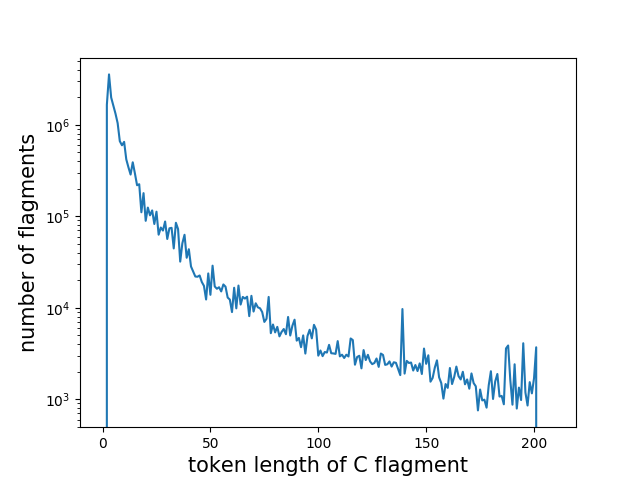
\includegraphics[width=12cm]{c_lens.png}
	\caption{Length distribution of C token flagments}
	\label{fig:csizes}
	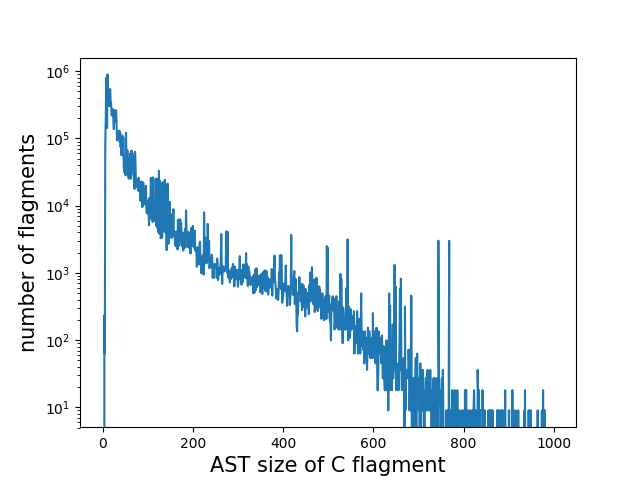
\includegraphics[width=12cm]{ast_lens.png}
	\caption{Length distribution of datasets as AST}
	\label{fig:astsizes}
\end{figure}

Figure~\ref{fig:csizes} shows the length distribution of the dataset as C token sequences
, and figure~\ref{fig:astsizes} shows the size distribution of the same dataset as ASTs.
The size of a AST is equals to the length of its action sequence.
According to the two figures, the AST size is 2~3 times larger than the length of C token sequences.
Therefore, the AST estimation may be harder than C token sequence estimation.

\begin{figure}
	\begin{tabular}{|l|l|} \hline
	 ground truth & 
		\begin{lstlisting}[style=Csample]
r *= a
		\end{lstlisting} \\ \hline
		Seq2Seq & 
		\begin{lstlisting}[style=Csample]
const unsigned int V0 = V1 * floatliteral
		\end{lstlisting} \\ \hline
		Seq2SeqAtt & 
		\begin{lstlisting}[style=Csample]
V0 = ( unsigned int ) ( V1 ) * ( unsigned int ) V2
		\end{lstlisting} \\ \hline
		Seq2Tree & 
		\begin{lstlisting}[style=Csample]
V0 = V0 * V1
		\end{lstlisting} \\ \hline
		\hline	
	 ground truth & 
		\begin{lstlisting}[style=Csample]
while(p >= 0){
	p--;
	r *= a;
}
		\end{lstlisting} \\ \hline
		Seq2Seq & 
		\begin{lstlisting}[style=Csample]
for(;V0 = (1<<(((unsigned int)-1<<((32-20)-1))-1))
*((unsigned char*)(V1.V2))[1] = (unsigned char)2;
}
		\end{lstlisting} \\ \hline
		Seq2SeqAtt & 
		\begin{lstlisting}[style=Csample]
while(((void *) >= 0) != ((void *) 0)){ 
	return ((void *) 0);
} else { 
	V0 = (( void * ) 0); 
}
		\end{lstlisting} \\ \hline
		Seq2Tree & 
		\begin{lstlisting}[style=Csample]
while(V0 < 0){ 
	V1 = V0 - 1;
}
		\end{lstlisting}
		 \\ \hline	\hline
	 ground truth & 
		\begin{lstlisting}[style=Csample]
int pow(int a,int p){
	int r = 1;
	while(p >= 0){
		p--;
		r *= a;
	}
	return r;
}
		\end{lstlisting} \\ \hline
		Seq2Seq & 
		\begin{lstlisting}[style=Csample]
void V0(int V1,int V1){ 
	int V1 = 0; 
	int V1; 
	for(V2=1;V1<=V2;++V2){ 
		V1 = * V3; 
	} 
}
		\end{lstlisting} \\ \hline
		Seq2SeqAtt & 
		\begin{lstlisting}[style=Csample]
void V0(unsigned int V1,unsigned int V2){ 
	unsigned int V1 = ((void *) 0); 
	unsigned int V3 = ((void *) 0); 
	unsigned int V1 = ((((void *) 0) != ((void *) 0))); 
	return V4; 
}
	\end{lstlisting} \\ \hline
		Seq2Tree & 
		\begin{lstlisting}[style=Csample]
INVALID_FUNCTION_DECL { 
	TRANCATETRANCATE 
}
		\end{lstlisting}
		 \\ \hline	
	\end{tabular}
	\caption{Smaple translation results for each model}
	\label{fig:sampletranse}
\end{figure}


\section{Sampled Decompilation Results}

Figure~\ref{fig:sampletranse} shows sample translate results for each model.

For the first short example, each of the models recovered that the C statement is composed of multiplication and assignment,
while only Seq2Tree recovered the name of the variables, and Seq2Seq and Seq2SeqAtt were failed to recover.

For the second middle example, Seq2Seq outputs invalid parenthesesed souce code, Seq2SeqAtt outputs invalid syntax (combination of while and else statement) code,
while Seq2Tree outputs correct syntax but many wrong subexpressions.

For the third large exapmle, all of the three models output a function with wrong body statement.
The {\sl INVALID\_FUNCTION\_DECL} in the result of Seq2Tree means it outputs wrong structured function type, and the {\sl TRANCATE} means 
the action is truncated because the too long action sequence is estimated. 
For long size function or statements, Seq2Tree tends to expand list type node to {\sl CONS} node, which causes infinit expansion of sequence,
and as a result, the type of the output function becomes broken and the body of the function becoms truncated.

According to these decompilation results, it can be said that these models is not acceptable for practical use.

% According to the figure 1, the 
% 図1からわかるように、attention付きのネットワークとそうでないネットワークの間には有意に差が存在しているが、
% Seq2seqWithAattention,Seq2Tree の間にはあまり差がみられない。

% 図3はSeq2Treeについて、木の大きさと正確さをプロットしたグラフである。

% (TODO)seq2seq、アテンション付きseq2seq、seq2treeとバイナリそのまま/逆アセンブル後 の6パターンのデータを出す。

% Figure~\ref{fig:csrs_lens} and figure~\ref{fig:ast_lens} show 学習に用いたデータセットについて、C言語のトークン列としてみたときのデータ長とAST tree として見たときの action size をそれぞれグラフにしてプロットしたものである。
% 全体的に、

% \section{Furure work}

\chapter{Furure research}
In this chapter, we suggest some other approaches to improve the accuracy of our decompilation models.

\section{Improvement on Assembly Code Preprocessing}
We used tokenized assembly string sequences for training. 
However, such simple concatnation of sequences might lose the information of the unity of each instructions.
To improve this point, we propose the following method.

This method uses two LSTM networks, the instruction encoder network and the assembly code encoder network, for encoding assembly token sequences.
First, each assembly instruction sequences are encoded by instruction encoding network into one instruction embedding vector, 
so that the assembly codes turn into the sequennces of embedding vectors.
Then, the sqeuence of embedding vectors is encoded into one reduced vector by assembly code encoder network.

This method will be time consuming compared to the method used in the experiment, however, this might be worth trying.

\section{Improvement on Sequence-to-tree Model}
We considered that the AST representation seems to exploit the feature of C source code. 
However, the sequence-to-tree model was not well performed.
In this section, we seek to the improvement of the AST approach.
\subsection{Copy Leaf Data from Assembler}
The translation results show that the sequence-to-tree model have difficalty in recovering the leaf data of the program.
Hence changing the method for expanding leaf node might improve the accuracy of decompilation.
There are three kind of leaf data in the AST representation of a C source code.

The first kind is the literal data. In the C source code, there are four literal data, integer, float, char and string. 
In the assembly code, the string literal appears in the form of a memory address, and the other three literals appear in the form of an immediate value.
Therefore, instead of estimating literal value directly, estimating the correcponding position in the assembly code might improve the correctness of decompilation.

The second kind is the type of operator. These can be also estimated from the assembly code.
For example, the operator $ + $ is compiled to the opecode {\sl add}, the operator $ | $ is compiled to the opecode {\sl or}, and so on. 
Thus the type of operator might be estimated by indicating the correspond position in the assembly code.

The third kind is the variable name. In the assembly code, a variable corresponds to a memory access. 
Therefore, the name of a variable is identified by its corresponding memory position, similar to avobe two kinds.

\subsection{Path Estimation} 
In the sequence-to-tree model, a tree structure is flattened into an action sequence, 
therefore the information of a tree structure might be lost in some degree.
For example, the adjacent actions in the action sequence might be the distant actions in the AST, when they are in the different subtree of the AST.

To preserve the information of the tree structure, we suddest to train the network for estimating each root-to-leaf action sequences in the AST,
instead of the flattened action sequence. 
For example, in the figure~\ref{fig:ast_zu}, there are four root-to-leaf action sequences, 
$ [act_1, act_2] $, $ [act_1, act_3,act_4,act_5,act_6,act_7] $, $ [act_1, act_3,act_4,act_8] $ and $ [act_1, act_3,act_4,act_9,act_{10}] $.
The AST can be recovered from these sequences instead of the whole sequence $ [act_1 \dots act_{10}] $, 
and these sequences are independent of each other, when generating AST.
Therefore, we may estimate each of the sequences from the asssembly token sequence by the sequence-to-sequence model.

This approach will ease the AST size problem, because the length of a root-to-leaf path is shorter than the size of whole AST, unless the AST has no branching.




% 前述の Sequence-to-Tree は プログラムの構造を考慮しているものの、アクションをそのまま列にするのは結局プログラムの木としての構造がある程度失われてしまっているのではないかと考えられる。
% すなわち、アクションを列に展開しているため、ある部分木からその兄弟の部分木の生成に移る際に大幅なジャンプが生じている。



\section{Improvement of Dataset}
As is seen in the figure~\ref{fig:csizes} and figure~\ref{fig:astsizes}, most of the data are short length C code.
This is due to our data generation method, which enumerates all of the subtree of a C source code.
We intended the models to learn the structure of long data from the short data, though the result shows that 
the poor decompilation results are generated from the longer data.
Therefore, the length distribution of the training data might effect on the training result, 
thus we will need to seek effective distribution for the training.


% \section{For General Decompiler}



\chapter{Conclusion}
We tested three neural network models Seq2Seq, Seq2SeqAtt and Seq2Tree for decompilation.
Numerically, Seq2SeqAtt peformanced better results compared to the other two models,
but all of three models were not acceptable for practical use.
Therefore, we will continue to develop practical decompiler for the good future of malware analysis.

\chapter{Acknowledgement}

\bibliographystyle{plainnat}
\bibliography{reference}

\end{document}
